% Copyright (C) 2020 Diogo Rodrigues, Breno Pimentel
% Distributed under the terms of the GNU General Public License, version 3

\documentclass[a4paper, 11pt]{report}
\usepackage[top=35mm,bottom=35mm,left=25mm,right=25mm]{geometry} % Margins

% Change section numbers
\renewcommand{\thesection}{\arabic{section}}

% Second page
\usepackage{secondpage}
\usepackage{datetime}

% Appendix
\usepackage{appendix}

% Landscape pages
\usepackage{pdflscape}
\usepackage{multicol}
\setlength\columnsep{50pt}

% Decent underlines
\usepackage[normalem]{ulem}

% Hyper-references
\usepackage{hyperref}

% Imports
\usepackage{import}

% Graphics and images
\usepackage{graphicx} \graphicspath{{./images/}}
\usepackage{tikz}
\usepackage{tikz-qtree}
\usetikzlibrary{automata, positioning, shapes, arrows}
\usepackage[justification=centering,font=small,skip=0.5em]{caption}
\usepackage{subcaption}
\usepackage{float}

\usepackage[binary-units=true]{siunitx} %SI units
\usepackage{pgfplots}
\pgfplotsset{compat=newest} % Allows to place the legend below plot
\usepgfplotslibrary{units} % Allows to enter the units nicely
\sisetup{
  round-mode          = places,
  round-precision     = 2,
}

% Encodings (to render letters with diacritics and special characters)
\usepackage[utf8]{inputenc}
% \DeclareUnicodeCharacter{2192}{\dash}

% Language
\usepackage[english]{babel}

% Source code and algorithms
%\usepackage{amsmath}
\usepackage{algorithm}
\usepackage[noend]{algpseudocode}
\usepackage{listings, chngcntr}
\lstset{
	basicstyle=\linespread{0.85}\ttfamily,
	basewidth  = {0.50em,1em},
    frame=tbr, % draw frame at top and bottom of the code
    tabsize=4, % tab space width
    numbers=left, % display line numbers on the left
	showstringspaces=false, % don't mark spaces in strings    
    commentstyle=\color{green}, % comment color
    keywordstyle=\color{blue}, % keyword color
    stringstyle=\color{red}, % string color
    breaklines=true,
    postbreak=\mbox{\textcolor{red}{$\hookrightarrow$}\space}
}
\lstdefinelanguage{cisco}{
    keywords = {
        enable,
        copy, reload,
        configure, terminal, end, interface, switchport, mode,
        access, vlan, show, interfaces, ip, address,
        no, shutdown, exit, nat, inside, outside, route, list, permit,
        pool, source, ovrld, overload, running, id
    },
    morecomment = [l]{\#}
}


% Tables with bold rows
\usepackage{tabularx}
\newcommand\setrow[1]{\gdef\rowmac{#1}#1\ignorespaces}
\newcommand\clearrow{\global\let\rowmac\relax}
\clearrow
\usepackage{multirow}
\usepackage{longtable}

% Tables with vertical center alignment
\usepackage{array}

% Lists and items
\usepackage[inline]{enumitem}

% Math stuff
\usepackage[mathscr]{euscript}
\usepackage{amssymb, latexsym} %Load math symbols like \blacksquare, but also load normal \leadsto arrows
\usepackage{mathtools} % For \text{...}
% \usepackage{enumitem}
% \usepackage{xcolor}
\newcommand{\expnumber}[2]{{#1}\mathrm{e}{#2}} % scientific notation
\newcommand{\degree}{^{\circ}}
\newcommand*\xor{\oplus}
\newcommand\expected[1]{\mathbf{E}[#1]}

% Headers and footers
\usepackage{fancyhdr}
\pagestyle{fancyplain}
\fancyhf{}
\lhead{\fancyplain{}{Configuration of a computer network — Report (RCOM 2020/21)}}
\rhead{\fancyplain{}{Class 2, group 4}}
\lfoot{\fancyplain{}{\leftmark}}
\rfoot{\thepage}

% Email
\newcommand{\email}[1]{
{\texttt{\href{mailto:#1}{#1}} }
}

% Metadata
\title{\Huge Configuration and study of a \\ computer network \\ \vspace*{12pt} \Large Report \\ \vspace*{4pt} \large FEUP - RCOM 2020/21}
\author{
Class 2, group 4 \vspace{0.5em} \\
\begin{tabular}{r l}
	\email{up201800170@fe.up.pt} & Breno Accioly de Barros Pimentel \\
	\email{up201806429@fe.up.pt} & Diogo Miguel Ferreira Rodrigues  \\
\end{tabular}
}
\date{23rd of December, 2020}

% Document
\begin{document}
\maketitle
\begin{secondpage}
    Copyright \copyright 2020--\the\year\ Diogo Rodrigues, Breno Pimentel\par
    \IfFileExists{VERSION}{Version \input{VERSION}}{Draft version}\par
    \immediate\write18{./get-commit-info.sh > COMMIT.tex}
    Built on \today~\currenttime~from \href{https://github.com/dmfrodrigues/feup-rcom-l2}{dmfrodrigues/feup-rcom-l2}, commit \input{COMMIT}\unskip.\par
    Permission is granted to copy and distribute this document under the terms of the
    \href{https://creativecommons.org/licenses/by-nc-nd/4.0/}{Creative Commons Attribution-NonCommercial-NoDerivatives 4.0 International}
    public license.
\end{secondpage}
\clearpage

\pagenumbering{arabic}

\section*{Summary}

This project was elaborated as the second project in the context of the curricular unit Computer Networks (RCOM), part of the Integrated Master in Informatics and Computing Engineering (MIEIC) at the Faculty of Engineering of the University of Porto (FEUP).
It concerns the configuration of a computer network, and its test and study through a developed FTP client.

All objectives were fulfilled, as we successfully implemented in C a simple FTP client for file retrieval over the Internet, and the configured network abided to the guidelines' requirements.

\section*{Introduction} \label{sec:Introduction}

The present project aims at developing a simple FTP client which is to be tested over a configured network.
The source code was developed in the C language, targeting Linux devices.
The goal network is composed of three computers, a switch that implements two virtual sub-networks, and a router to provide Internet access.

This report describes the corresponding project's activities, and is divided into two parts.
In part 1 we address the design, development and testing of the FTP client.
In part 2 we describe the steps on configuring the computer network, over the course of seven short experiments that incrementally contribute to the final network configuration.
This project was tested in the computers of FEUP, room I321, bench 3, with rack computers 2, 3 and 4, a Cisco Catalyst 3560 Series switch and a Cisco 2900 Series router.

\section{Download application} \label{sec:Part1}

A simple FTP client was developed to test the network configuration.

\subsection{Application architecture} \label{sec:Arc}

The application first parses and verifies if the URL abides to \cite{rfc1738} using a regular expression (\texttt{ftp://[<user>:<password>@]<host>/<url-path>}).
Then it finds the IP address with a call to \texttt{gethostbyname} and the application opens a connection using a socket through port 21 to the FTP server. 

After connecting, it logs in to the server, or otherwise logs in as anonymous if no credentials were provided.
Next, it sends a \texttt{PASV} command to the FTP server so it can transfer data in passive mode; if successful, the server will reply
with six bytes, the first four being the server IP address it just opened for transfer, and the other two the port the server is listening on. 

After entering passive mode, the download application opens another socket, using the port provided by the server, where the data will be transferred.
Finally, it copies the file from \texttt{<url-path>} to the current working directory and finishes the connection by sending the \texttt{QUIT} command and closing the sockets.

To build the application, run \texttt{make} in directory \texttt{download}. To test the application, run:

\begin{lstlisting}[frame=none, numbers=none, language=sh]
./download ftp://[<user>:<password>@]<host>/<url-path>
\end{lstlisting}


\subsection{Report of successful download} \label{sec:Dow}

The application was tested in different FTP servers, with files varying in size and type, with and without credentials.
Reports can be found in \ref{listing:6-2-tux33-pipe}, \ref{listing:6-2-tux33-pic2}, \ref{listing:6-5-tux32} and \ref{listing:6-5-tux33}.

\section{Network configuration and analysis} \label{sec:Part2}

\subsection{Experiment 1} \label{sec:Exp1}

\begin{figure}[H]
	\centering
    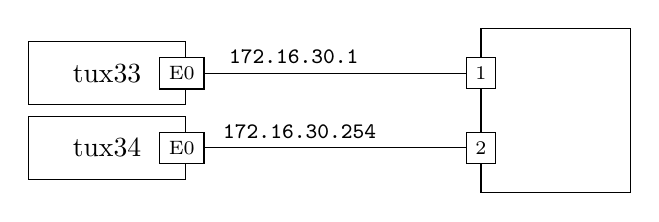
\begin{tikzpicture}[-,>=stealth',node distance=2cm,initial text=$ $,scale=0.95]
        \node at (0,-0) [rectangle,draw,minimum height=0.8cm, minimum width=2cm] (tux33) {tux33};
        \node at (1.0, -0) [rectangle, draw, fill=white] (tux33_E0){ \scriptsize E0 };

        \node at (0,-1.0) [rectangle,draw, minimum height=0.8cm, minimum width=2cm] (tux34) {tux34};
        \node at (1.0, -1) [rectangle, draw, fill=white] (tux34_E0){ \scriptsize E0 };
        


        \draw   (5, +0.6) rectangle ++(2, -2.2);
        \node at (5.0, -0.00) [rectangle, draw, fill=white] (switch_1){ \scriptsize 1 };
        \node at (5.0, -1.00) [rectangle, draw, fill=white] (switch_2){ \scriptsize 2 };

        \draw   (tux33_E0)    edge[above, align=left]     node[xshift=-0.45cm]{\footnotesize \texttt{172.16.30.1  }}          (switch_1)
                (tux34_E0)    edge[above, align=left]     node[xshift=-0.45cm]{\footnotesize \texttt{172.16.30.254}}          (switch_2)
            ;
    \end{tikzpicture}
	\caption{Network architecture for experiment 1}
	\label{fig:network_exp1}
\end{figure}

\noindent
\textbf{Objectives:} connect two computers by configuring their IP addresses.

\subsubsection{Main configuration commands} \label{sec:Com1}

\begin{tabular}{l | p{75mm} | l}
    \textbf{Dev.} & \textbf{Description}                                  & \textbf{Commands}                       \\ \hline
    tux33         & Activate \texttt{eth0} interface                     & \texttt{ifconfig eth0 up}               \\
    tux33         & Set \texttt{eth0} IP 172.16.30.1, with 24-bit mask   & \texttt{ifconfig eth0 172.16.30.1/24}   \\ \hline
    tux34         & Activate \texttt{eth0} interface                     & \texttt{ifconfig eth0 up}               \\
    tux34         & Set \texttt{eth0} IP 172.16.30.254, with 24-bit mask & \texttt{ifconfig eth0 172.16.30.254/24} \\
\end{tabular}

\subsubsection{Logs analysis} \label{sec:Log1}

IP (Internet Protocol) addresses are a convenient way to refer to interfaces, but to send a frame a device first needs to know the MAC address of the receiving interface.
ARP (Address Resolution Protocol) is used to map an IP address to a MAC address; these mappings are stored in the ARP table, and each device has one such table.
Upon sending a frame, if there is not an entry with the receiver IP in its ARP table, the emitter will broadcast an ARP probe packet with the receiver IP and wait for the corresponding device to announce its presence.

As per log \ref{listing:1-10-tux33.pcapng}, tux33 broadcasts an ARP request in packet \#9 for the desired IP address \texttt{172.16.30.254}.
Then tux34 identifies itself, sending to tux33 another ARP packet with its MAC address \texttt{00:21:5a:5a:7d:74} in packet \#10.

\texttt{ping} generates ICMP (Internet Control Message Protocol) packets. The MAC/IP addresses of the ping packets are the source addresses \texttt{00:21:5a:61:24:92}/\texttt{172.16.30.1} in bytes 0-5
and destination addresses in bytes 6-11 \texttt{00:21:5a:7d:74}/\texttt{172.16.30.254}.

A ARP and IPv4 frames can be identified with the type value 0x806 and 0x800 respectively in the Ethernet II layer.
It is possible to determine if a receiving Ethernet frame have a ICMP layer by checking its IPv4 field and verifying the value 0x01 in the protocol byte.
We could also determine the length of a Ethernet frame by adding the 14 bytes of the Ethernet II layer to the total length described in the IPv4 layer for ICMP packets.
In the case of a ARP packet, the request length is found by adding the Ethernet II layer length and the ARP layer length, the reply length is the previous sum but with a additional padding length. 

The loopback interface allows access to the almost-discontinued Ethernet Configuration Testing Protocol (CTP)\cite{how-ethernet-keepalive-works}\cite[ch.~8]{ethernet}, with provides services similar to \texttt{ping} but on the Data Link layer \cite{jhawk}. It is implemented at least in Cisco routers \cite{jhawk}\cite{whats-a-loop-traffic-in-ethereal} and the switch software configuration guide \cite{cisco-switch-manual} does mention the loopback interface although it does not clearly explain what it is. Due to its specifications, this interface/protocol can serve any of the following purposes:
\begin{enumerate*}[label=(\arabic*)]
    \item \label{itm:connectivity} test connectivity with another station;
    \item \label{itm:loops} check for network loops;
    \item \label{itm:own-issues} check for hardware issues by sending a request to itself \cite{whats-a-loop-traffic-in-ethereal};
    \item \label{itm:self-loop} check for self-looped ports.
\end{enumerate*}
Although CTP was primarily designed for \ref{itm:connectivity} \cite[sec.~8.1]{ethernet}, Cisco now only implements CTP for purposes \ref{itm:own-issues} and \ref{itm:self-loop}\cite{whats-a-loop-traffic-in-ethereal}. In our case it probably serves \ref{itm:self-loop}, as the loopback packets in \ref{listing:1-10-tux33.pcapng} have their source and destination MAC addresses set to those of the device which is consistent with \cite{whats-a-loop-traffic-in-ethereal}. We assume that if the packets were to serve purpose \ref{itm:own-issues} they would not actually be sent down the line, but rather through some internal physical or software medium. As such, computers should just ignore that specific packet, whether or not they implement CTP (if a device does not implement CTP, which is the case for most devices and all mainstream OSs, it will ignore all LOOP requests either way). These packets are sent every 10 seconds.

\subsection{Experiment 2} \label{sec:Exp2}

\begin{figure}[H]
	\centering
    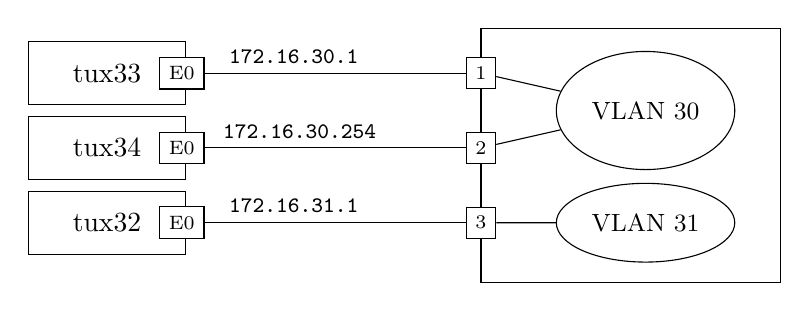
\begin{tikzpicture}[-,>=stealth',node distance=2cm,initial text=$ $,scale=0.95]
        \node at (0,-0) [rectangle,draw,minimum height=0.8cm, minimum width=2cm] (tux33) {tux33};
        \node at (1.0, -0) [rectangle, draw, fill=white] (tux33_E0){ \scriptsize E0 };

        \node at (0,-1.0) [rectangle,draw, minimum height=0.8cm, minimum width=2cm] (tux34) {tux34};
        \node at (1.0, -1) [rectangle, draw, fill=white] (tux34_E0){ \scriptsize E0 };
        
        \node at (0,-2) [rectangle,draw, minimum height=0.8cm, minimum width=2cm] (tux32) {tux32};
        \node at (1.0, -2) [rectangle, draw, fill=white] (tux32_E0){ \scriptsize E0 };

        \draw   (5, +0.6) rectangle ++(4, -3.4);
        \node at (7.2, -0.5) [ellipse, draw, minimum height = 1.5cm, minimum width = 2.0cm, align=center] (VLAN30) {\small VLAN 30};
        \node at (7.2, -2.0) [ellipse, draw, minimum height = 1.0cm, minimum width = 2.0cm, align=center] (VLAN31) {\small VLAN 31};
        \node at (5.0, -0.00) [rectangle, draw, fill=white] (switch_1){ \scriptsize 1 };
        \node at (5.0, -1.00) [rectangle, draw, fill=white] (switch_2){ \scriptsize 2 };
        \node at (5.0, -2.00) [rectangle, draw, fill=white] (switch_3){ \scriptsize 3 };

        \draw   (tux33_E0)    edge[above, align=left]     node[xshift=-0.45cm]{\footnotesize \texttt{172.16.30.1  }}          (switch_1)
                (tux34_E0)    edge[above, align=left]     node[xshift=-0.45cm]{\footnotesize \texttt{172.16.30.254}}          (switch_2)
                (tux32_E0)    edge[above, align=left]     node[xshift=-0.45cm]{\footnotesize \texttt{172.16.31.1  }}          (switch_3)
                
                (switch_1) edge[] (VLAN30)
                (switch_2) edge[] (VLAN30)
                (switch_3) edge[] (VLAN31)
            ;

    \end{tikzpicture}
	\caption{Network architecture for experiment 2}
	\label{fig:network_exp2}
\end{figure}

\noindent
\textbf{Objectives:} implement two virtual LANs in a switch.

\subsubsection{Main configuration commands} \label{sec:Com2}

\begin{tabular}{l | p{75mm} | l}
    \textbf{Dev.} & \textbf{Description}                                  & \textbf{Commands}                       \\ \hline
    switch        & Create virtual LAN 30                                 &
        \begin{lstlisting}[frame=none, numbers=none, language=sh]
configure terminal
vlan 30
end
        \end{lstlisting} \\
    switch        & Assign port 1 to VLAN 30                              & 
        \begin{lstlisting}[frame=none, numbers=none, language=sh]
configure terminal
interface fastethernet 0/1
switchport mode access
switchport access vlan 30
end
        \end{lstlisting} \\
\end{tabular}

\subsubsection{Logs analysis} \label{sec:Log2}

To configure VLAN30, we had to create it in the switch, and then add switch port 1 (tux33-E0) and switch port 2 (tux34-E0) to that VLAN.

From log \ref{listing:2-5-tux33.pcapng} we infer tux33 can ping tux34 but cannot ping tux32 (the failed pings to tux32 are not in the log, but we have experimentally verified this outcome from \texttt{ping} output).
From logs \ref{listing:2-7-tux32.pcapng}, \ref{listing:2-7-tux33.pcapng} and \ref{listing:2-7-tux34.pcapng} we see that a broadcast from tux33 can reach tux33 and tux34, but not tux32.
From logs \ref{listing:2-10-tux32.pcapng}, \ref{listing:2-10-tux33.pcapng} and \ref{listing:2-10-tux34.pcapng} we see that a broadcast from tux32 can only reach tux32.
This leads us to conclude there are two virtual networks, VLAN30 which includes tux33 and tux34, and VLAN31 which includes tux32, as well as that there are two different broadcast domains, one for each subnet: \texttt{172.16.31.255} and \texttt{172.16.30.255}.

Upon close inspection of logs \ref{listing:2-7-tux33.pcapng} and \ref{listing:2-7-tux34.pcapng}, it can be seen that the destination of the broadcast issued from tux33 is \texttt{172.16.30.0}.
We tried to analyse this issue, and concluded the most likely option is that we issued the broadcast from tux33 to the wrong IP address (\texttt{172.16.30.0} instead of the obvious broadcast address \texttt{172.16.30.255} for VLAN30), but that somehow the ping was still considered a broadcast as it is also obvious this ping reached tux34.
There are some \cite{ping-subnet-address-1}\cite{ping-subnet-address-2} who mention that historically some devices treat the subnet IP address as a broadcast address.

On inspecting the ping requests, both broadcasts sent from tux33 and tux32 are Ethernet II frames have their destination set to the MAC broadcast address \texttt{ff:ff:ff:ff:ff:ff}, and only the contained IPv4 destination addresses differ.
The switch works on the Data Link layer so it can only understand the Ethernet II frames, not the contained IPv4 packet so it broadcasts both pings in exactly the same way, each in its own subnetwork; so apparently, somewhere in the process of converting the destination IP address to a MAC address, tux33 interpreted \texttt{172.16.30.0} as a broadcast address and framed the IPv4 packet in a frame destined to the MAC broadcast address \texttt{ff:ff:ff:ff:ff:ff}. This is further reinforced by the fact even the \texttt{ping} command recognizes a network address as a broadcast address, assumed from its output \texttt{ping: Do you want to ping broadcast? Then -b. If not, check your local firewall rules} when you try to ping a network IP address without using the \texttt{-b} (broadcast) flag. 

\subsection{Experiment 3} \label{sec:Exp3}

\begin{figure}[H]
	\centering
    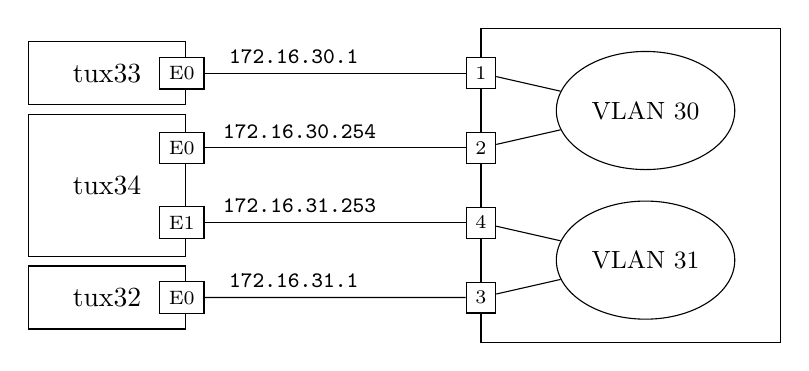
\begin{tikzpicture}[-,>=stealth',node distance=2cm,initial text=$ $,scale=0.95]
        \node at (0,-0) [rectangle,draw,minimum height=0.8cm, minimum width=2cm] (tux33) {tux33};
        \node at (1.0, -0) [rectangle, draw, fill=white] (tux33_E0){ \scriptsize E0 };

        \node at (0,-1.5) [rectangle,draw, minimum height=1.8cm, minimum width=2cm] (tux34) {tux34};
        \node at (1.0, -1) [rectangle, draw, fill=white] (tux34_E0){ \scriptsize E0 };
        \node at (1.0, -2) [rectangle, draw, fill=white] (tux34_E1){ \scriptsize E1 };
        
        \node at (0,-3) [rectangle,draw, minimum height=0.8cm, minimum width=2cm] (tux32) {tux32};
        \node at (1.0, -3) [rectangle, draw, fill=white] (tux32_E0){ \scriptsize E0 };

        \draw   (5, +0.6) rectangle ++(4, -4.2);
        \node at (7.2, -0.5) [ellipse, draw, minimum height = 1.5cm, minimum width = 2.0cm, align=center] (VLAN30) {\small VLAN 30};
        \node at (7.2, -2.5) [ellipse, draw, minimum height = 1.5cm, minimum width = 2.0cm, align=center] (VLAN31) {\small VLAN 31};
        \node at (5.0, -0.00) [rectangle, draw, fill=white] (switch_1){ \scriptsize 1 };
        \node at (5.0, -1.00) [rectangle, draw, fill=white] (switch_2){ \scriptsize 2 };
        \node at (5.0, -2.00) [rectangle, draw, fill=white] (switch_4){ \scriptsize 4 };
        \node at (5.0, -3.00) [rectangle, draw, fill=white] (switch_3){ \scriptsize 3 };

        \draw   (tux33_E0)    edge[above, align=left]     node[xshift=-0.45cm]{\footnotesize \texttt{172.16.30.1  }}          (switch_1)
                (tux34_E0)    edge[above, align=left]     node[xshift=-0.45cm]{\footnotesize \texttt{172.16.30.254}}          (switch_2)
                (tux32_E0)    edge[above, align=left]     node[xshift=-0.45cm]{\footnotesize \texttt{172.16.31.1  }}          (switch_3)
                (tux34_E1)    edge[above, align=left]     node[xshift=-0.45cm]{\footnotesize \texttt{172.16.31.253}}          (switch_4)

                (switch_1) edge[] (VLAN30)
                (switch_2) edge[] (VLAN30)
                (switch_3) edge[] (VLAN31)
                (switch_4) edge[] (VLAN31)
            ;

    \end{tikzpicture}
	\caption{Network architecture for experiment 3}
	\label{fig:network_exp3}
\end{figure}

\textbf{Objectives:} configure a router in Linux.

\subsubsection{Main configuration commands} \label{sec:Com3}

\begin{tabular}{l | p{43mm} | l}
    \textbf{Dev.} & \textbf{Description}                                  & \textbf{Commands}                       \\ \hline
    tux34         & Configure tux34-E1 [was associated to eth2 (\textbf{!})] &
        \begin{lstlisting}[frame=none, numbers=none, language=sh]
ifconfig eth2 up
ifconfig eth2 172.16.31.253/24
        \end{lstlisting} \\
    tux34         & Enable IP forwarding & 
    \begin{lstlisting}[frame=none, numbers=none, language=sh]
echo 1 > /proc/sys/net/ipv4/ip_forward
    \end{lstlisting} \\
    tux34         & Disable ICMP echo-ignore-broadcast &  
    \begin{lstlisting}[frame=none, numbers=none, language=sh]
echo 0 > /proc/sys/net/ipv4/
    icmp_echo_ignore_broadcasts
    \end{lstlisting} \\ \hline
    tux32         & Add route to VLAN30 &  
    \begin{lstlisting}[frame=none, numbers=none, language=sh]
route add -net 172.16.30.0/24 gw 172.16.31.253
    \end{lstlisting} \\ \hline
    tux33         & Add route to VLAN31 &  
    \begin{lstlisting}[frame=none, numbers=none, language=sh]
route add -net 172.16.31.0/24 gw 172.16.30.254
    \end{lstlisting} \\ \hline
    switch        & Add port 4 to VLAN 31 & 
    \begin{lstlisting}[frame=none, numbers=none, language=sh]
configure terminal
interface fastethernet 0/4
switchport mode access
switchport access vlan 31
end
    \end{lstlisting}
\end{tabular}

\subsubsection{Logs analysis} \label{sec:Log3}

\begin{center}
    \small
    \begin{tabular}{l | l}
        \textbf{Dev.} & \begin{lstlisting}[basicstyle=\linespread{0.85}\ttfamily\footnotesize, frame=, numbers=none]
Destination     Gateway         Genmask         Flags Metric Ref    Use Iface
            \end{lstlisting} \\ \hline
        tux32 & \lstinputlisting[basicstyle=\linespread{0.85}\ttfamily\small, frame=, numbers=none, firstline=3]{../../part2/exp3/3-4-tux32.route.txt} \\ \hline
        tux33 & \lstinputlisting[basicstyle=\linespread{0.85}\ttfamily\small, frame=, numbers=none, firstline=3]{../../part2/exp3/3-4-tux33.route.txt} \\ \hline
        tux34 & \lstinputlisting[basicstyle=\linespread{0.85}\ttfamily\small, frame=, numbers=none, firstline=3]{../../part2/exp3/3-4-tux34.route.txt}
    \end{tabular}
\end{center}

A forwarding table entry contains the destination address, a gateway where the data will be redirected, the netmask used, flags, metric, references, use and the network interface.

It is possible to observe in the logs the ARP message requesting for the gateway address 172.16.30.254 when running the ping command in tux33 to tux32.
This happens because this is the next hop in the route, through there it can be redirected to the final destination.

We are able to observe ICMP packets between all computers in the network, meaning all of them are connected.

When running the ping command from tux33 to tux32, the source MAC address is from tux33 but the destination MAC address is from tux34. This also happens because tux34
work as a gateway between both VLANs.

\subsection{Experiment 4} \label{sec:Exp4}

\begin{figure}[H]
	\centering
    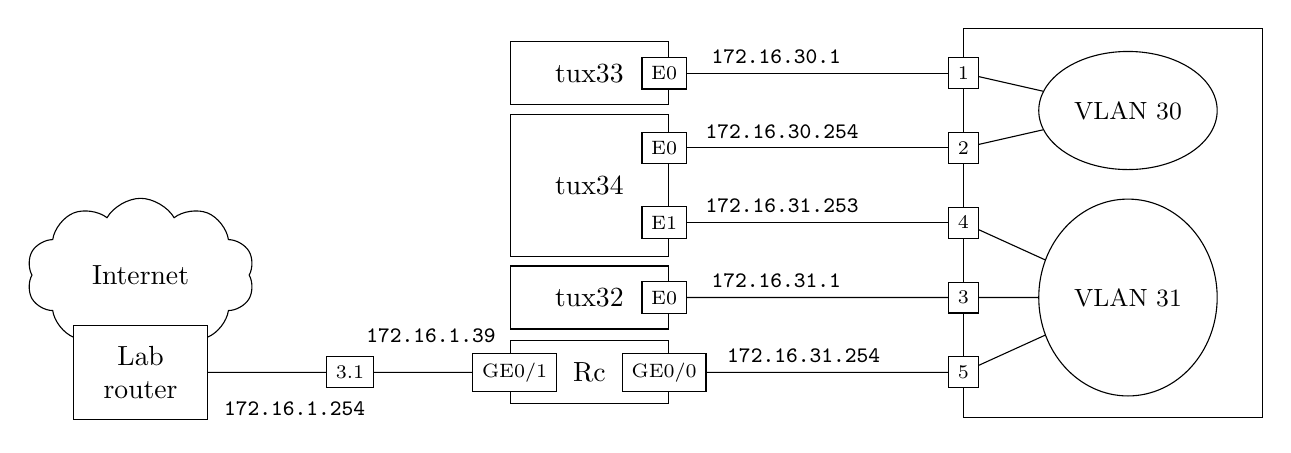
\begin{tikzpicture}[-,>=stealth',node distance=2cm,initial text=$ $,scale=0.95]
        \node at (0,-0) [rectangle,draw,minimum height=0.8cm, minimum width=2cm] (tux33) {tux33};
        \node at (1.0, -0) [rectangle, draw, fill=white] (tux33_E0){ \scriptsize E0 };

        \node at (0,-1.5) [rectangle,draw, minimum height=1.8cm, minimum width=2cm] (tux34) {tux34};
        \node at (1.0, -1) [rectangle, draw, fill=white] (tux34_E0){ \scriptsize E0 };
        \node at (1.0, -2) [rectangle, draw, fill=white] (tux34_E1){ \scriptsize E1 };
        
        \node at (0,-3) [rectangle,draw, minimum height=0.8cm, minimum width=2cm] (tux32) {tux32};
        \node at (1.0, -3) [rectangle, draw, fill=white] (tux32_E0){ \scriptsize E0 };

        \node at (0,-4) [rectangle,draw, minimum height=0.8cm, minimum width=2cm] (Rc) {Rc};
        \node at (1.0, -4) [rectangle, draw, fill=white] (Rc_GE0){ \scriptsize GE0/0 };
        \node at (-1.0, -4) [rectangle, draw, fill=white] (Rc_GE1){ \scriptsize GE0/1 };

        \node at (-3.2, -4) [rectangle, draw, fill=white] (3_1){ \scriptsize 3.1 };

        \node at (-6,-2.7) [cloud, draw,cloud puffs=10,cloud puff arc=120, aspect=1.8, inner ysep=1.2em] {Internet};
        \node at (-6,-4) [rectangle,draw, minimum height=1.2cm, minimum width=1.7cm, align=center, fill=white] (lab_router) {Lab\\router};

        \draw   (5, +0.6) rectangle ++(4, -5.2);
        \node at (7.2, -0.5) [ellipse, draw, minimum height = 1.5cm, minimum width = 2.0cm, align=center] (VLAN30) {\small VLAN 30};
        \node at (7.2, -3.0) [ellipse, draw, minimum height = 2.5cm, minimum width = 2.0cm, align=center] (VLAN31) {\small VLAN 31};
        \node at (5.0, -0.00) [rectangle, draw, fill=white] (switch_1){ \scriptsize 1 };
        \node at (5.0, -1.00) [rectangle, draw, fill=white] (switch_2){ \scriptsize 2 };
        \node at (5.0, -2.00) [rectangle, draw, fill=white] (switch_4){ \scriptsize 4 };
        \node at (5.0, -3.00) [rectangle, draw, fill=white] (switch_3){ \scriptsize 3 };
        \node at (5.0, -4.00) [rectangle, draw, fill=white] (switch_5){ \scriptsize 5 };

        \draw   (tux33_E0)    edge[above, align=left]     node[xshift=-0.45cm]{\footnotesize \texttt{172.16.30.1  }}          (switch_1)
                (tux34_E0)    edge[above, align=left]     node[xshift=-0.45cm]{\footnotesize \texttt{172.16.30.254}}          (switch_2)
                (tux32_E0)    edge[above, align=left]     node[xshift=-0.45cm]{\footnotesize \texttt{172.16.31.1  }}          (switch_3)
                (tux34_E1)    edge[above, align=left]     node[xshift=-0.45cm]{\footnotesize \texttt{172.16.31.253}}          (switch_4)
                (Rc_GE0)      edge[above, align=left]     node[xshift=-0.30cm]{\footnotesize \texttt{172.16.31.254}}          (switch_5)
                (Rc_GE1)      edge[above, align=right]    node[xshift=+0.10cm, yshift=+0.25cm]{\footnotesize \texttt{172.16.1.39}}            (3_1)
                (3_1)         edge[below, align=left]     node[xshift=+0.35cm, yshift=-0.25cm]{\footnotesize \texttt{172.16.1.254}}          (lab_router)

                (switch_1) edge[] (VLAN30)
                (switch_2) edge[] (VLAN30)
                (switch_3) edge[] (VLAN31)
                (switch_4) edge[] (VLAN31)
                (switch_5) edge[] (VLAN31)
            ;

    \end{tikzpicture}
	\caption{Network architecture for experiment 4}
	\label{fig:network_exp4}
\end{figure}

\textbf{Objectives:} configure a commercial router and implement NAT.

\subsubsection{Main configuration commands} \label{sec:Com4}
\subsubsection{Logs analysis} \label{sec:Log4}

When running the ping command from tux32 to tux33 without redirects, the packets first arrived on the router and then were redirected to tux34 and after it tux33.
After enabling the redirects and running ping again, the router sends a ICMP redirect message to tux32 that allows tux32 to directly send packets to tux34, without needing to go first through the router.

NAT is a method to translate IP addresses of computers in a network to a single public IP address.

\subsection{Experiment 5} \label{sec:Exp5}

\begin{figure}[H]
	\centering
    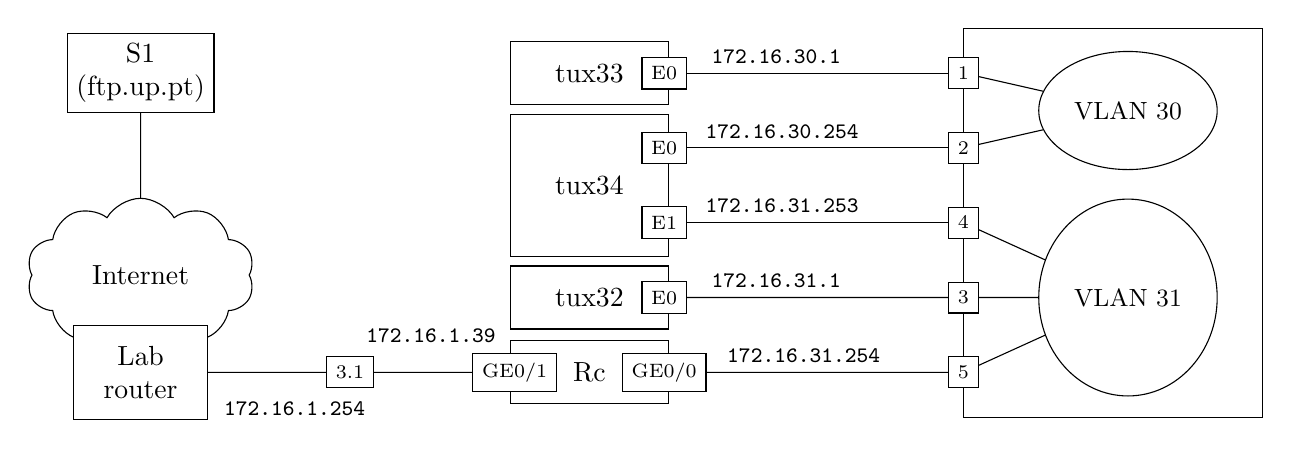
\begin{tikzpicture}[-,>=stealth',node distance=2cm,initial text=$ $,scale=0.95]
        \node at (0,-0) [rectangle,draw,minimum height=0.8cm, minimum width=2cm] (tux33) {tux33};
        \node at (1.0, -0) [rectangle, draw, fill=white] (tux33_E0){ \scriptsize E0 };

        \node at (0,-1.5) [rectangle,draw, minimum height=1.8cm, minimum width=2cm] (tux34) {tux34};
        \node at (1.0, -1) [rectangle, draw, fill=white] (tux34_E0){ \scriptsize E0 };
        \node at (1.0, -2) [rectangle, draw, fill=white] (tux34_E1){ \scriptsize E1 };
        
        \node at (0,-3) [rectangle,draw, minimum height=0.8cm, minimum width=2cm] (tux32) {tux32};
        \node at (1.0, -3) [rectangle, draw, fill=white] (tux32_E0){ \scriptsize E0 };

        \node at (0,-4) [rectangle,draw, minimum height=0.8cm, minimum width=2cm] (Rc) {Rc};
        \node at (1.0, -4) [rectangle, draw, fill=white] (Rc_GE0){ \scriptsize GE0/0 };
        \node at (-1.0, -4) [rectangle, draw, fill=white] (Rc_GE1){ \scriptsize GE0/1 };

        \node at (-3.2, -4) [rectangle, draw, fill=white] (3_1){ \scriptsize 3.1 };

        \node at (-6,-2.7) [cloud, draw,cloud puffs=10,cloud puff arc=120, aspect=1.8, inner ysep=1.2em] (internet) {Internet};
        \node at (-6,-4) [rectangle,draw, minimum height=1.2cm, minimum width=1.7cm, align=center, fill=white] (lab_router) {Lab\\router};

        \node at (-6, -0) [rectangle,draw, minimum height=1.0cm, minimum width=1.7cm, align=center, fill=white] (dns_server) {S1\\(ftp.up.pt)};

        \draw   (5, +0.6) rectangle ++(4, -5.2);
        \node at (7.2, -0.5) [ellipse, draw, minimum height = 1.5cm, minimum width = 2.0cm, align=center] (VLAN30) {\small VLAN 30};
        \node at (7.2, -3.0) [ellipse, draw, minimum height = 2.5cm, minimum width = 2.0cm, align=center] (VLAN31) {\small VLAN 31};
        \node at (5.0, -0.00) [rectangle, draw, fill=white] (switch_1){ \scriptsize 1 };
        \node at (5.0, -1.00) [rectangle, draw, fill=white] (switch_2){ \scriptsize 2 };
        \node at (5.0, -2.00) [rectangle, draw, fill=white] (switch_4){ \scriptsize 4 };
        \node at (5.0, -3.00) [rectangle, draw, fill=white] (switch_3){ \scriptsize 3 };
        \node at (5.0, -4.00) [rectangle, draw, fill=white] (switch_5){ \scriptsize 5 };

        \draw   (tux33_E0)    edge[above, align=left]     node[xshift=-0.45cm]{\footnotesize \texttt{172.16.30.1  }}          (switch_1)
                (tux34_E0)    edge[above, align=left]     node[xshift=-0.45cm]{\footnotesize \texttt{172.16.30.254}}          (switch_2)
                (tux32_E0)    edge[above, align=left]     node[xshift=-0.45cm]{\footnotesize \texttt{172.16.31.1  }}          (switch_3)
                (tux34_E1)    edge[above, align=left]     node[xshift=-0.45cm]{\footnotesize \texttt{172.16.31.253}}          (switch_4)
                (Rc_GE0)      edge[above, align=left]     node[xshift=-0.30cm]{\footnotesize \texttt{172.16.31.254}}          (switch_5)
                (Rc_GE1)      edge[above, align=right]    node[xshift=+0.10cm, yshift=+0.25cm]{\footnotesize \texttt{172.16.1.39}}            (3_1)
                (3_1)         edge[below, align=left]     node[xshift=+0.35cm, yshift=-0.25cm]{\footnotesize \texttt{172.16.1.254}}          (lab_router)

                (switch_1) edge[] (VLAN30)
                (switch_2) edge[] (VLAN30)
                (switch_3) edge[] (VLAN31)
                (switch_4) edge[] (VLAN31)
                (switch_5) edge[] (VLAN31)
                (dns_server) edge[] (internet)
            ;

    \end{tikzpicture}
	\caption{Network architecture for experiment 5}
	\label{fig:network_exp4}
\end{figure}

\textbf{Objectives:} Configure DNS service.

\subsubsection{Main configuration commands} \label{sec:Com5}
\begin{tabular}{p{11mm} | p{26mm} | p{112mm}}
    \textbf{Dev.} & \textbf{Description}                                  & \textbf{Commands}                       \\ \hline
    tux32, tux33, tux34      & Configure DNS & 
    \begin{lstlisting}[frame=none, numbers=none, language=sh, aboveskip=-0.5 \baselineskip, belowskip=-0.8 \baselineskip]
echo -e "search netlab.fe.up.pt\nnameserver 172.16.1.1" > /etc/resolv.conf
    \end{lstlisting}
\end{tabular}
\subsubsection{Logs analysis} \label{sec:Log5}

After tux33 (172.16.30.1) sent a query to the DNS server services.netlab.fe.up.pt (172.16.1.1),
in our logs for www.sapo.pt, 172.16.1.1 sent a query response with the corresponding IP address 213.13.146.142.
This IP address was used afterwards by tux33 to send ICMP packets.

\subsection{Experiment 6} \label{sec:Exp6}
\begin{figure}[H]
	\centering
    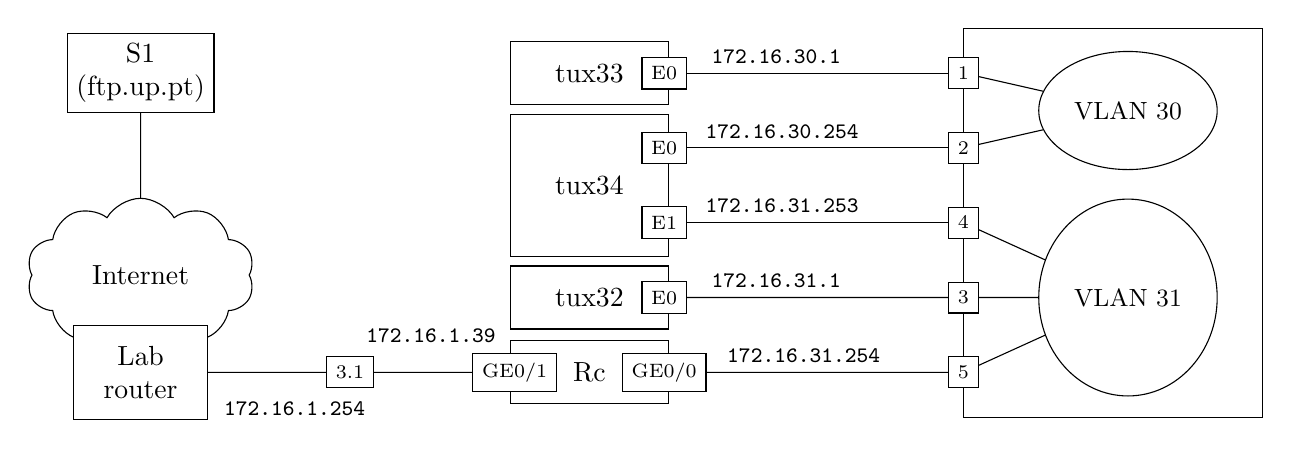
\begin{tikzpicture}[-,>=stealth',node distance=2cm,initial text=$ $,scale=0.95]
        \node at (0,-0) [rectangle,draw,minimum height=0.8cm, minimum width=2cm] (tux33) {tux33};
        \node at (1.0, -0) [rectangle, draw, fill=white] (tux33_E0){ \scriptsize E0 };

        \node at (0,-1.5) [rectangle,draw, minimum height=1.8cm, minimum width=2cm] (tux34) {tux34};
        \node at (1.0, -1) [rectangle, draw, fill=white] (tux34_E0){ \scriptsize E0 };
        \node at (1.0, -2) [rectangle, draw, fill=white] (tux34_E1){ \scriptsize E1 };
        
        \node at (0,-3) [rectangle,draw, minimum height=0.8cm, minimum width=2cm] (tux32) {tux32};
        \node at (1.0, -3) [rectangle, draw, fill=white] (tux32_E0){ \scriptsize E0 };

        \node at (0,-4) [rectangle,draw, minimum height=0.8cm, minimum width=2cm] (Rc) {Rc};
        \node at (1.0, -4) [rectangle, draw, fill=white] (Rc_GE0){ \scriptsize GE0/0 };
        \node at (-1.0, -4) [rectangle, draw, fill=white] (Rc_GE1){ \scriptsize GE0/1 };

        \node at (-3.2, -4) [rectangle, draw, fill=white] (3_1){ \scriptsize 3.1 };

        \node at (-6,-2.7) [cloud, draw,cloud puffs=10,cloud puff arc=120, aspect=1.8, inner ysep=1.2em] (internet) {Internet};
        \node at (-6,-4) [rectangle,draw, minimum height=1.2cm, minimum width=1.7cm, align=center, fill=white] (lab_router) {Lab\\router};

        \node at (-6, -0) [rectangle,draw, minimum height=1.0cm, minimum width=1.7cm, align=center, fill=white] (dns_server) {S1\\(ftp.up.pt)};

        \draw   (5, +0.6) rectangle ++(4, -5.2);
        \node at (7.2, -0.5) [ellipse, draw, minimum height = 1.5cm, minimum width = 2.0cm, align=center] (VLAN30) {\small VLAN 30};
        \node at (7.2, -3.0) [ellipse, draw, minimum height = 2.5cm, minimum width = 2.0cm, align=center] (VLAN31) {\small VLAN 31};
        \node at (5.0, -0.00) [rectangle, draw, fill=white] (switch_1){ \scriptsize 1 };
        \node at (5.0, -1.00) [rectangle, draw, fill=white] (switch_2){ \scriptsize 2 };
        \node at (5.0, -2.00) [rectangle, draw, fill=white] (switch_4){ \scriptsize 4 };
        \node at (5.0, -3.00) [rectangle, draw, fill=white] (switch_3){ \scriptsize 3 };
        \node at (5.0, -4.00) [rectangle, draw, fill=white] (switch_5){ \scriptsize 5 };

        \draw   (tux33_E0)    edge[above, align=left]     node[xshift=-0.45cm]{\footnotesize \texttt{172.16.30.1  }}          (switch_1)
                (tux34_E0)    edge[above, align=left]     node[xshift=-0.45cm]{\footnotesize \texttt{172.16.30.254}}          (switch_2)
                (tux32_E0)    edge[above, align=left]     node[xshift=-0.45cm]{\footnotesize \texttt{172.16.31.1  }}          (switch_3)
                (tux34_E1)    edge[above, align=left]     node[xshift=-0.45cm]{\footnotesize \texttt{172.16.31.253}}          (switch_4)
                (Rc_GE0)      edge[above, align=left]     node[xshift=-0.30cm]{\footnotesize \texttt{172.16.31.254}}          (switch_5)
                (Rc_GE1)      edge[above, align=right]    node[xshift=+0.10cm, yshift=+0.25cm]{\footnotesize \texttt{172.16.1.39}}            (3_1)
                (3_1)         edge[below, align=left]     node[xshift=+0.35cm, yshift=-0.25cm]{\footnotesize \texttt{172.16.1.254}}          (lab_router)

                (switch_1) edge[] (VLAN30)
                (switch_2) edge[] (VLAN30)
                (switch_3) edge[] (VLAN31)
                (switch_4) edge[] (VLAN31)
                (switch_5) edge[] (VLAN31)
                (dns_server) edge[] (internet)
            ;

    \end{tikzpicture}
	\caption{Network architecture for experiment 5}
	\label{fig:network_exp4}
\end{figure}

\textbf{Objectives:} Test the download application in the configured network.

\subsubsection{Main configuration commands} \label{sec:Com6}
\subsubsection{Logs analysis} \label{sec:Log6}

The download application opened two TCP connections. 
The first was used through port 21 to send and receive commands to the server, this connection is responsible for the FTP control information.
The second was opened in the port specified after entering passive mode, this was used to transfer data between the server and the client.

A TCP connection is divided in three phases. 
In the first phase a connection is stablished with a three-way handshake, a SYN command is sent to the server, the server then replies with a SYN-ACK and the client sends ACK to the server.
In the second phase happens the data-transfer.
In the third phase is another three-way handshake, the client sends a FIN, the server replies with FIN-ACK and the client ends with ACK. 

The TCP uses the method ARQ (Automatic Repeat Request) to handle errors in the data-transfer.
This method sends ACK (acknowlegdment message) when the data is received successfully before a timeout occurs.
If a timeout does occurs, the data is retransmitted until it is correctly received.

The TCP also have a congestion control mechanism, which uses a congestion window that limits the amount of data this protocol can send into the network, 
so it does not send more than the window size field (specified in bytes) that can be found in the TCP header. 

\section*{Conclusion} \label{sec:Conclusion}

\bibliographystyle{acm}
\addcontentsline{toc}{section}{Bibliography}
\bibliography{report}

\appendix
\appendixpage
\addappheadtotoc
\chapter{Source code}

The source code of this project can be obtained from \href{https://github.com/dmfrodrigues/feup-rcom-l2}{github.com/dmfrodrigues/feup-rcom-l2}.
The source code is made available by \textcopyright~Diogo Rodrigues and Breno Pimentel under the \href{https://www.gnu.org/licenses/gpl-3.0.en.html}{GNU General Public License v3} (GPLv3), which you should have received together with the source code, or that you can otherwise obtain online.

During project development and evaluation the repository remained private, although it can be shared with evaluators on request to clarify the development process or due to other justifiable reasons.
It will be made public once all equivalent curricular unit projects have been evaluated in the present school year.

\newgeometry{top=24mm,bottom=24mm,left=14mm,right=14mm}
\fancyhfoffset{0pt}

\lstinputlisting[basicstyle=\ttfamily\small, caption=\texttt{url\_parser.h}, language=C]{../../download/include/url_parser.h}
\lstinputlisting[basicstyle=\ttfamily\small, caption=\texttt{url\_parser.c}, language=C]{../../download/src/url_parser.c}

\lstinputlisting[basicstyle=\ttfamily\small, caption=\texttt{server\_cmds.h}, language=C]{../../download/include/server_cmds.h}
\lstinputlisting[basicstyle=\ttfamily\small, caption=\texttt{server\_cmds.c}, language=C]{../../download/src/server_cmds.c}

\lstinputlisting[basicstyle=\ttfamily\small, caption=\texttt{download.h}, language=C]{../../download/include/download.h}
\lstinputlisting[basicstyle=\ttfamily\small, caption=\texttt{download.c}, language=C]{../../download/src/download.c}

\restoregeometry

\chapter{Configuration commands}
\lstinputlisting[basicstyle=\ttfamily\small, caption=\texttt{tuxy2\_config.sh}, language=bash]{../../part2/config/tuxy2_config.sh}
\lstinputlisting[basicstyle=\ttfamily\small, caption=\texttt{tuxy3\_config.sh}, language=bash]{../../part2/config/tuxy3_config.sh}
\lstinputlisting[basicstyle=\ttfamily\small, caption=\texttt{tuxy4\_config.sh}, language=bash]{../../part2/config/tuxy4_config.sh}
\lstinputlisting[basicstyle=\ttfamily\small, caption=\texttt{switch.sh}, language=cisco]{../../part2/config/switch.sh}
\lstinputlisting[basicstyle=\ttfamily\small, caption=\texttt{router.sh}, language=cisco]{../../part2/config/router.sh}

\newgeometry{top=24mm,bottom=24mm,left=14mm,right=14mm}
\fancyhfoffset{0pt}
\chapter{Logs}

\counterwithin{lstlisting}{subsection}
\renewcommand{\thelstlisting}{%
  \thechapter.\thesubsection(\arabic{lstlisting})%
}

\begin{center}
    \begin{tabular}{l | l | l}
        \textbf{Interface} & \textbf{MAC address}       & \texttt{IP address}    \\ \hline
        tux32-eth0         & \texttt{00:21:5a:61:30:63} & \texttt{172.16.31.1  } \\
        tux33-eth0         & \texttt{00:21:5a:61:24:92} & \texttt{172.16.30.1  } \\
        tux34-eth0         & \texttt{00:21:5a:5a:7d:74} & \texttt{172.16.30.254} \\
        tux34-eth2         & \texttt{00:c0:df:25:26:0a} & \texttt{172.16.31.253} \\
        Rc-GE0/0           & \texttt{                 } & \texttt{172.16.31.254} \\
        Rc-GE0/1           & \texttt{                 } & \texttt{172.16.1.39  } \\
    \end{tabular}
\end{center}

\section{Experiment 1}
\setcounter{subsection}{4}
\subsection{Item 5}
\lstinputlisting[basicstyle=\linespread{0.85}\ttfamily\small, frame=tbr, caption=\texttt{1-5-tux33-routes.txt}]{../../part2/exp1/1-5-tux33-routes.txt}
\lstinputlisting[basicstyle=\linespread{0.85}\ttfamily\small, frame=tbr, caption=\texttt{1-5-tux33-arp.txt}   ]{../../part2/exp1/1-5-tux33-arp.txt}
\lstinputlisting[basicstyle=\linespread{0.85}\ttfamily\small, frame=tbr, caption=\texttt{1-5-tux34-routes.txt}]{../../part2/exp1/1-5-tux34-routes.txt}
\lstinputlisting[basicstyle=\linespread{0.85}\ttfamily\small, frame=tbr, caption=\texttt{1-5-tux34-arp.txt}   ]{../../part2/exp1/1-5-tux34-arp.txt}

\begin{landscape}
\setcounter{subsection}{9}
\subsection{Item 10}
\lstinputlisting[basicstyle=\linespread{0.85}\ttfamily\scriptsize, frame=tbr, label={listing:1-10-tux33.pcapng}, caption=\texttt{1-10-tux33.pcapng.txt}]{../../part2/exp1/1-10-tux33.pcapng.txt}
\end{landscape}

\begin{landscape}
\section{Experiment 2}

\setcounter{subsection}{4}
\subsection{Item 5}
\lstinputlisting[basicstyle=\linespread{0.85}\ttfamily\scriptsize, frame=tbr, label={listing:2-5-tux33.pcapng}, caption=\texttt{2-5-tux33.pcapng.txt}]{../../part2/exp2/2-5-tux33.pcapng.txt} \pagebreak

\setcounter{subsection}{6}
\subsection{Item 7}

\lstinputlisting[basicstyle=\linespread{0.85}\ttfamily\scriptsize, frame=tbr, label={listing:2-7-tux32.pcapng}, caption=\texttt{2-7-tux32.pcapng.txt}]{../../part2/exp2/2-7-tux32.pcapng.txt} \pagebreak
\lstinputlisting[basicstyle=\linespread{0.85}\ttfamily\scriptsize, frame=tbr, label={listing:2-7-tux33.pcapng}, caption=\texttt{2-7-tux33.pcapng.txt}]{../../part2/exp2/2-7-tux33.pcapng.txt} \pagebreak
\lstinputlisting[basicstyle=\linespread{0.85}\ttfamily\scriptsize, frame=tbr, label={listing:2-7-tux34.pcapng}, caption=\texttt{2-7-tux34.pcapng.txt}]{../../part2/exp2/2-7-tux34.pcapng.txt} \pagebreak

\setcounter{subsection}{9}
\subsection{Item 10}

\lstinputlisting[basicstyle=\linespread{0.85}\ttfamily\scriptsize, frame=tbr, label={listing:2-10-tux32.pcapng}, caption=\texttt{2-10-tux32.pcapng.txt}]{../../part2/exp2/2-10-tux32.pcapng.txt} \pagebreak
\lstinputlisting[basicstyle=\linespread{0.85}\ttfamily\scriptsize, frame=tbr, label={listing:2-10-tux33.pcapng}, caption=\texttt{2-10-tux33.pcapng.txt}]{../../part2/exp2/2-10-tux33.pcapng.txt} \pagebreak
\lstinputlisting[basicstyle=\linespread{0.85}\ttfamily\scriptsize, frame=tbr, label={listing:2-10-tux34.pcapng}, caption=\texttt{2-10-tux34.pcapng.txt}]{../../part2/exp2/2-10-tux34.pcapng.txt}
\end{landscape}

\begin{landscape}
\section{Experiment 3}

\setcounter{subsection}{2}
\subsection{Item 3}
\lstinputlisting[basicstyle=\linespread{0.85}\ttfamily\small, frame=tbr, caption=\texttt{3-7-tux32.route.txt}]{../../part2/exp3/3-4-tux32.route.txt}
\lstinputlisting[basicstyle=\linespread{0.85}\ttfamily\small, frame=tbr, caption=\texttt{3-7-tux33.route.txt}]{../../part2/exp3/3-4-tux33.route.txt}
\lstinputlisting[basicstyle=\linespread{0.85}\ttfamily\small, frame=tbr, caption=\texttt{3-7-tux34.route.txt}]{../../part2/exp3/3-4-tux34.route.txt}

\setcounter{subsection}{6}
\subsection{Item 7}

\lstinputlisting[basicstyle=\linespread{0.85}\ttfamily\scriptsize, frame=tbr, caption=\texttt{3-7-tux33.pcapng.txt}]{../../part2/exp3/3-7-tux33.pcapng.txt} \pagebreak

\setcounter{subsection}{7}
\subsection{Item 8}

\lstinputlisting[basicstyle=\linespread{0.85}\ttfamily\scriptsize, frame=tbr, caption=\texttt{3-8-tux34-eth0.pcapng.txt}]{../../part2/exp3/3-8-tux34-eth0.pcapng.txt} \pagebreak
\lstinputlisting[basicstyle=\linespread{0.85}\ttfamily\scriptsize, frame=tbr, caption=\texttt{3-8-tux34-eth1.pcapng.txt}]{../../part2/exp3/3-8-tux34-eth1.pcapng.txt}
\end{landscape}

\begin{landscape}
\section{Experiment 4}

\setcounter{subsection}{2}
\subsection{Item 3}
\lstinputlisting[basicstyle=\linespread{0.85}\ttfamily\scriptsize, frame=tbr, caption=\texttt{4-3-tux33.pcapng.txt}]{../../part2/exp4/4-3-tux33.pcapng.txt}

\setcounter{subsection}{3}
\subsection{Item 4}
\lstinputlisting[basicstyle=\linespread{0.85}\ttfamily\small     , frame=tbr, caption=\texttt{4-4c-tux32-noredirect-noroute.ping.txt}       ]{../../part2/exp4/4-4c-tux32-noredirect-noroute.ping.txt}
\lstinputlisting[basicstyle=\linespread{0.85}\ttfamily\scriptsize, frame=tbr, caption=\texttt{4-4c-tux32-noredirect-noroute.pcapng.txt}     ]{../../part2/exp4/4-4c-tux32-noredirect-noroute.pcapng.txt}
\end{landscape}

\begin{landscape}
\lstinputlisting[basicstyle=\linespread{0.85}\ttfamily\small     , frame=tbr, caption=\texttt{4-4e-tux32-noredirect-noroute.traceroute.txt} ]{../../part2/exp4/4-4e-tux32-noredirect-noroute.traceroute.txt}
\lstinputlisting[basicstyle=\linespread{0.85}\ttfamily\small     , frame=tbr, caption=\texttt{4-4f-tux32-noredirect-yesroute.traceroute.txt}]{../../part2/exp4/4-4f-tux32-noredirect-yesroute.traceroute.txt}
\lstinputlisting[basicstyle=\linespread{0.85}\ttfamily\small     , frame=tbr, caption=\texttt{4-4g-tux32-yesredirect-noroute.ping.txt}      ]{../../part2/exp4/4-4g-tux32-yesredirect-noroute.ping.txt}
\lstinputlisting[basicstyle=\linespread{0.85}\ttfamily\scriptsize, frame=tbr, caption=\texttt{4-4g-tux32-yesredirect-noroute.pcapng.txt}    ]{../../part2/exp4/4-4g-tux32-yesredirect-noroute.pcapng.txt}
\end{landscape}

\begin{landscape}
\setcounter{subsection}{4}
\subsection{Item 5}
\lstinputlisting[basicstyle=\linespread{0.85}\ttfamily\small     , frame=tbr, caption=\texttt{4-5-tux33.ping.txt}  ]{../../part2/exp4/4-5-tux33.ping.txt}
\lstinputlisting[basicstyle=\linespread{0.85}\ttfamily\scriptsize, frame=tbr, caption=\texttt{4-5-tux33.pcapng.txt}]{../../part2/exp4/4-5-tux33.pcapng.txt}
\end{landscape}

\begin{landscape}
\setcounter{subsection}{6}
\subsection{Item 7}
\lstinputlisting[basicstyle=\linespread{0.85}\ttfamily\small     , frame=tbr, caption=\texttt{4-7-tux33.ping.txt}  ]{../../part2/exp4/4-7-tux33.ping.txt}
\lstinputlisting[basicstyle=\linespread{0.85}\ttfamily\scriptsize, frame=tbr, caption=\texttt{4-7-tux33.pcapng.txt}]{../../part2/exp4/4-7-tux33.pcapng.txt}
\end{landscape}

\begin{landscape}
\section{Experiment 5}
\setcounter{subsection}{2}
\subsection{Item 3}
\lstinputlisting[basicstyle=\linespread{0.85}\ttfamily\small     , frame=tbr, caption=\texttt{5-3-tux33.ping.txt}  ]{../../part2/exp5/5-3-tux33.ping.txt}
\lstinputlisting[basicstyle=\linespread{0.85}\ttfamily\scriptsize, frame=tbr, caption=\texttt{5-3-tux33.pcapng.txt}]{../../part2/exp5/5-3-tux33.pcapng.txt}
\end{landscape}

\begin{landscape}
\section{Experiment 6}

\setcounter{subsection}{1}
\subsection{Item 2}
\subsubsection{Transferring \texttt{pipe.txt}}
\lstinputlisting[basicstyle=\linespread{0.85}\ttfamily\small, frame=tbr, label={listing:6-2-tux33-pipe}, caption=\texttt{6-2-tux33-pipe.download.txt}]{../../part2/exp6/6-2-tux33-pipe.download.txt}
\lstinputlisting[basicstyle=\linespread{0.85}\ttfamily\tiny , frame=tbr,                                 caption=\texttt{6-2-tux33-pipe.pcapng.txt}  ]{../../part2/exp6/6-2-tux33-pipe.pcapng.txt}
\end{landscape}

\begin{landscape}
\subsubsection{Transferring \texttt{pic2.png}}
\lstinputlisting[basicstyle=\linespread{0.85}\ttfamily\small, frame=tbr, label={listing:6-2-tux33-pic2}, caption=\texttt{6-2-tux33-pic2.download.txt}]{../../part2/exp6/6-2-tux33-pic2.download.txt}
\lstinputlisting[basicstyle=\linespread{0.85}\ttfamily\tiny , frame=tbr,                                 caption=\texttt{6-2-tux33-pic2.pcapng.txt}  ]{../../part2/exp6/6-2-tux33-pic2.pcapng.txt}
\end{landscape}

\begin{landscape}
\setcounter{subsection}{4}
\subsection{Item 5}
\lstinputlisting[basicstyle=\linespread{0.85}\ttfamily\small, frame=tbr, label={listing:6-5-tux32}, caption=\texttt{6-5-tux32.download.txt}]{../../part2/exp6/6-5-tux32.download.txt}
\lstinputlisting[basicstyle=\linespread{0.85}\ttfamily\tiny , frame=tbr,                            caption=\texttt{6-5-tux32.pcapng.txt}  ]{../../part2/exp6/6-5-tux32.pcapng.txt}
\end{landscape}

\begin{landscape}
\lstinputlisting[basicstyle=\linespread{0.85}\ttfamily\small, frame=tbr, label={listing:6-5-tux33}, caption=\texttt{6-5-tux33.download.txt}]{../../part2/exp6/6-5-tux33.download.txt}
\lstinputlisting[basicstyle=\linespread{0.85}\ttfamily\tiny , frame=tbr,                            caption=\texttt{6-5-tux33.pcapng.txt}  ]{../../part2/exp6/6-5-tux33.pcapng.txt}
\end{landscape}

\restoregeometry

\end{document}
